% latexmk -pvc -pdf
\documentclass[9pt, a4paper]{article}
\usepackage[margin=0.65in]{geometry}
\usepackage{graphicx}
\usepackage{caption}
\usepackage{amsmath,amsthm,amsfonts,amssymb}
\usepackage{blindtext}
\usepackage[english]{babel}
\newenvironment{Figure}
    {\par\medskip\noindent\minipage{\linewidth}}
    {\endminipage\par\medskip}

\title{Simulating phase contrast imaging for materials with variable density (PART II)}
\author{Ana C. Fabela Hinojosa \\
\small{Supervisors: Assoc. Prof. Marcus Kitchen}}
\small{\date{\today,  \\Due date: Friday 23\textsuperscript{th} September, 2021}}

\begin{document}
\maketitle
\section{Current objective}
In this project I study the theoretical perspective of coherent X-ray imaging. Presently I investigate via a simulation whether is possible to observe phase contrast from a sample of two different brain material samples of grey and white matter under the same wave-field.
My current simulations consider 2 cases: In the first case I assume the simulated materials are chemically identical but have distinct densities (hence the optical properties observed are strictly density dependent) and in the second case my assumptions are that the materials have different optical properties independent of density.  
I am trying to verify if and how distinctly phase contrast occurs. The eventual goal of this simulation is to verify if successful phase retrieval can be done of the imaged objects given their variable densities.
% The simulation that I am presently working on involves a two concentric cylinders made of two distinct materials (each with constant density). My supervisor and I are curious to see if we can verify a claim in one of the texts I am using in my research. This claim concerns a propagation based phase contrast imaging (PBI) algorithm that was first developed by Paganin et al. (2002)\cite{Pags2002}\cite{CH49}. Specifically, the claim states that the stability of Paganin's algorithm is thought to be dependent among other factors in the ratio between $\delta$ and $\mu$, both of which are proportional to the density of the medium. The conclusion from this claim is essentially that: any changes in material density throughout the material would not affect the imaging process. My supervisor suspects that this statement might not be entirely correct and we want to verify if the stability of the Paganin et al. (2002) algorithm is dependent instead on the ratio of the differences in the refraction and attenuation coefficients $\Delta \delta$ and $\Delta \mu$.

\section{Theory fundamentals}

One of my simulations uses the projection approximation to solve a partial differential equation known as the transport-of-intensity equation (TIE). The TIE physically describes the divergence of the transverse energy-flow vector known as the Poynting vector $(\textbf{S})$\cite{PagsTutes}.
\begin{equation}\label{eq:1}
-\nabla_{T} [I(x, y, z) \nabla_{T} \phi(x, y, z)] = k \frac{\partial I (x, y, z)}{\partial z}.
\end{equation}
where $k$ is the wave-number, $I(x, y, z)$ is the intensity and $\phi(x, y, z)$ is the phase of the X-ray beam, the Poynting vector $\textbf{S} \propto I(x, y, z) \nabla_{T} \phi(x, y, z)$.
The projection approximation assumes that X-ray flow may be well approximated by straight lines parallel to z\cite{PagsTutes} and that most X-rays passing through an object do not actually interact with the sample material, neglecting scattering effects is mathematically equivalent to discarding the transverse Laplacian term in equation (\ref{eq:1})\cite{CH49}, in addition X-ray--matter interaction must be taken into account. To do this the position dependent and complex form for the refractive index
is introduced: $n(x, y, z) = 1 - \delta(x, y, z) + i \beta(x, y, z)$, the real part of this complex quantity corresponds to the refractive index properties of the sample while the imaginary part is related only to the absorptive properties\cite{PagsTutes}.

The projection approximation results in the Beer-Lambert law of attenuation which relates the intensity attenuation to the properties of the sample
\begin{equation}\label{eq:2}
I(x, y, z_0) = \mathrm{exp}[-\int_{t} \mu(x, y, z) dz] I(x, y, 0),
\end{equation}
where $\mu = 2k\beta$ is the \textit{linear attenuation coefficient} of the sample.

The projection approximation term involving the refractive index $\delta$, quantifies the deformation of the X-ray wave-fronts due to passage through the sample object. Physically, this describes phase-shifts of each wave-front coordinate which continuously accumulate in the direction of the light propagation.
\begin{equation}\label{eq:3}
\Delta \phi(x, y) = -k \int_{t}\delta(x, y, z)dz,
\end{equation}
where $t$ is the projected thickness of the object in the direction of the light flow.

Once the intensity (equation \ref{eq:2}) and phase (equation \ref{eq:3}) of the scattered wave-field have been calculated at a z value immediately after the imaged sample(this corresponds to an (x, y) transverse plane to the direction of light propagation z). This transverse plane is conventionally known as the exit-surface plane. and is used as the initial conditions for the intensity and phase in the TIE.  The TIE propagation 
effects observable changes onto the intensity and phase of the exit-surface plane initial conditions, and so the sample can be studied using the imaging system. 


\section{Current progress and results}

Using the projection approximation to establish my initial conditions, I solved the TIE in two-dimensions for the case of a monomorphic material cylinder. My method used the fourth order Runge-Kutta evolution algorithm to propagate the intensity and phase that described the monochromatic scalar electromagnetic wave-field over a distance of 1 meter. Originally my code discretised a two-dimensional space as an x with 1021 points and a y array with 512 points. To calculate the wave-field's derivative terms in equation (\ref{eq:1}) I first attempted to solve the TIE in Fourier space by writing the derivative terms in the TIE using the Fourier derivative theorem. I defined functions describing the geometry and optical properties (i.e. refractive index: $\delta(x, y, z)$ and $\mu(x, y, z)$) of the simulated cylinder. Both $\delta$ and $\mu$ functions used a sigmoid function with adjustable gradient to slightly blur the edge of the cylinder and avoid instability while finding the initial conditions to be used in the TIE by solving the integrals in equations (\ref{eq:2}) and (\ref{eq:3}). My method was slow due to the Fourier derivatives and the output intensity profile after propagation did not appear very stable. I adjusted the ratio of the spacings in my discretised space several times to make sure that the Nyquist mode of the TIE was resolved adequately. Eventually I managed to get a smooth looking intensity profile.
\begin{Figure}
\centering
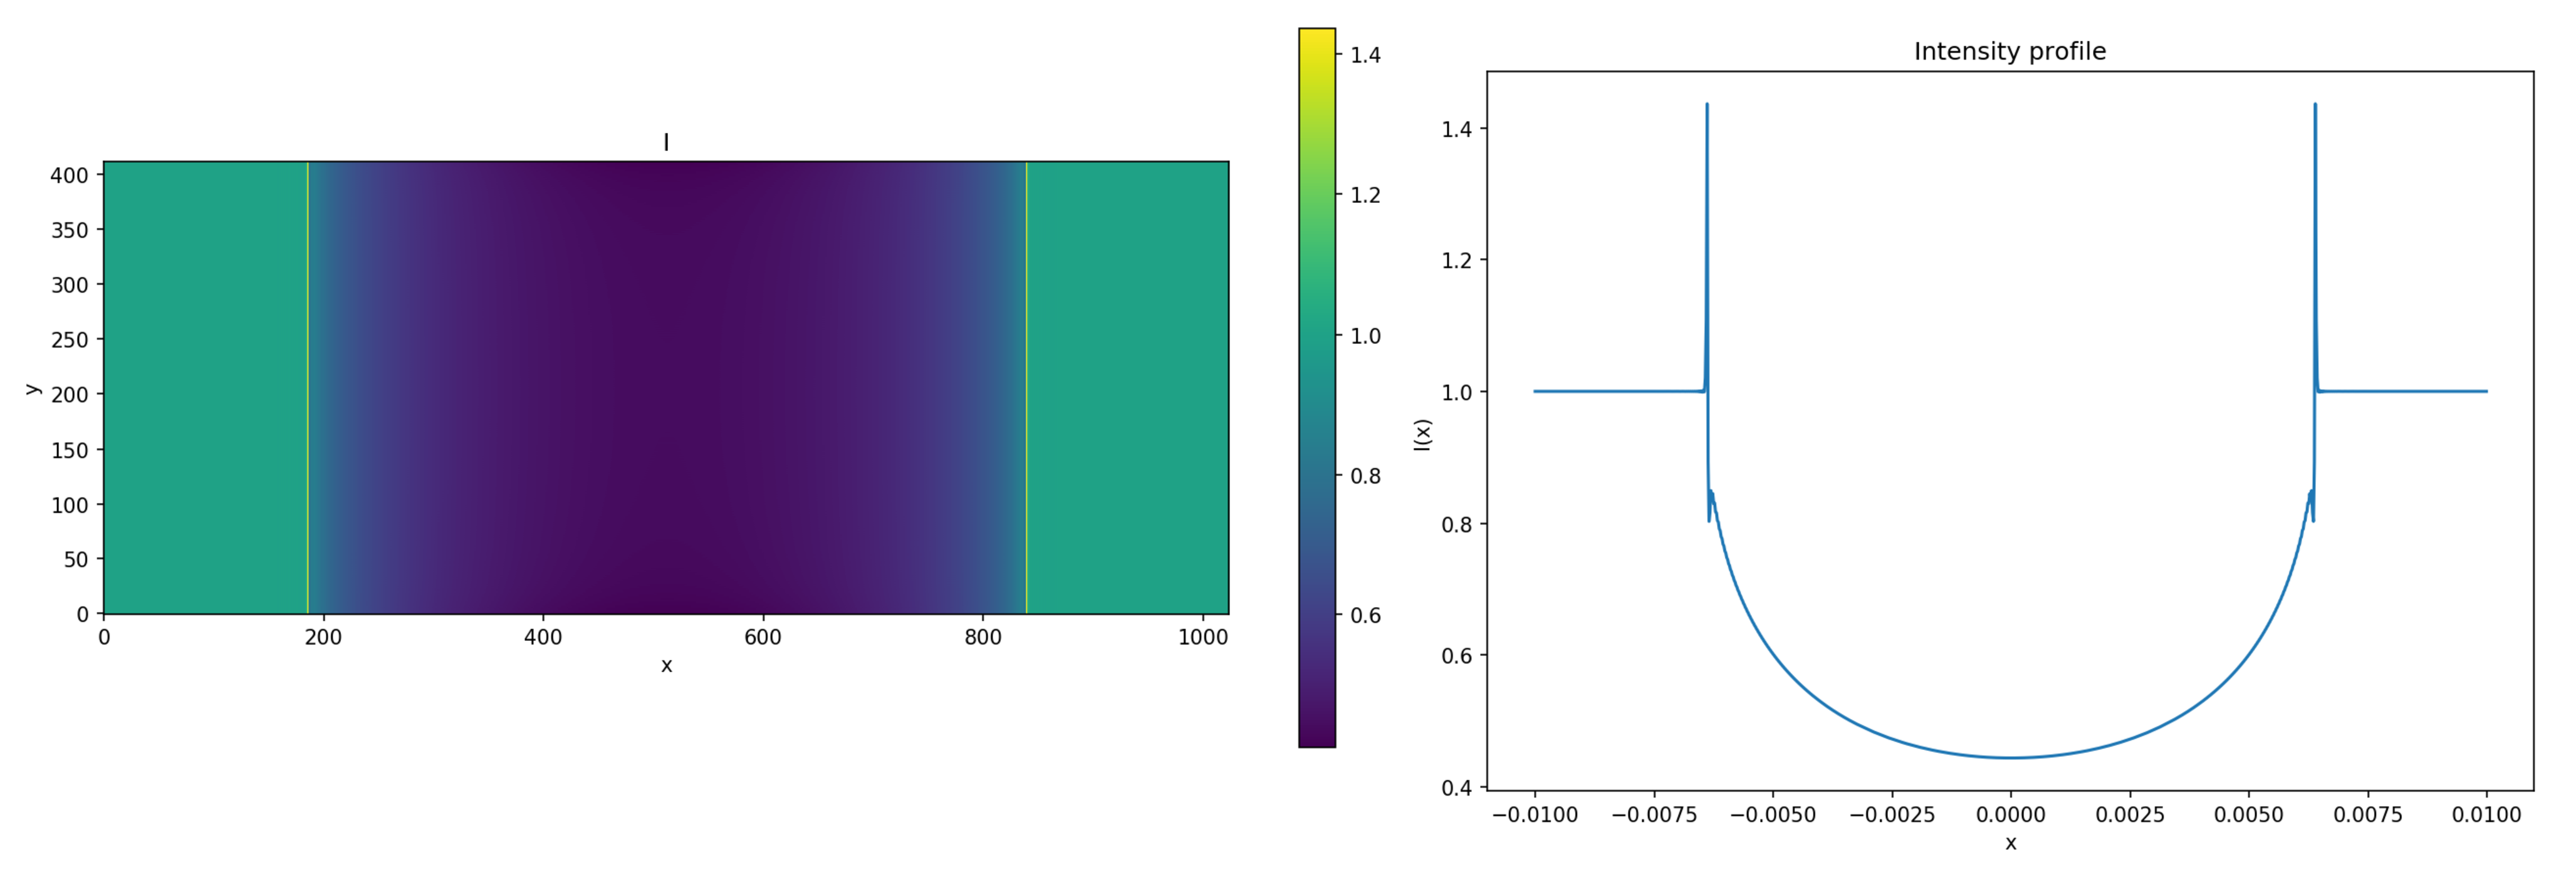
\includegraphics[width=\linewidth]{Fourier_intensity_profile.pdf}
\captionof{figure}{These phase contrast image and phase contrast cross section were the best results I obtained from my Fourier TIE method. Unfortunately my Fourier method was not able to simultaneously match the expected phase contrast peak height given the energy and sample material parameters while at the same time remaining stable. The parameters used to obtain this image were an X-ray energy equal to $22.1629$keV (corresponding to a Ag k-alpha 1 source), the cylinder's material was water which has a refractive index decrement $\delta_1 = 468.141$nm while the attenuation coefficient at this energy is $\mu_1 = 64.38436\mathrm{m^{-1}}$, the sigmoid function blurred 0.5 pixels over the edge of the imaged cylinder. The apparent asymmetry of the two-dimensional phase contrast image is due to aliasing.}
\end{Figure}

After this suboptimal result I decided to change my approach slightly and at the suggestion of my supervisor I used \texttt{numpy.gradient} for the derivative terms and \texttt{scipy.ndimage.laplace} for the phase Laplacian term in the TIE. This time my code discretised the two-dimensional space as an x and a y array each with 1024 points. 
After these changes I was able to understand the probable underlying reason why my Fourier method didn't work even though in theory it should have, given that it is accurate to infinite order\cite{Chris}\cite{Fornberg}. The issue was due to an effect known as Gibbs phenomenon, this effect occurs when the nth partial sum of a Fourier series undergoes large oscillations near regions with jump discontinuities\cite{Gibbs}. Discovering that higher degree polynomial interpolation does not always improve accuracy was certainly unexpected.
\begin{Figure}
\centering
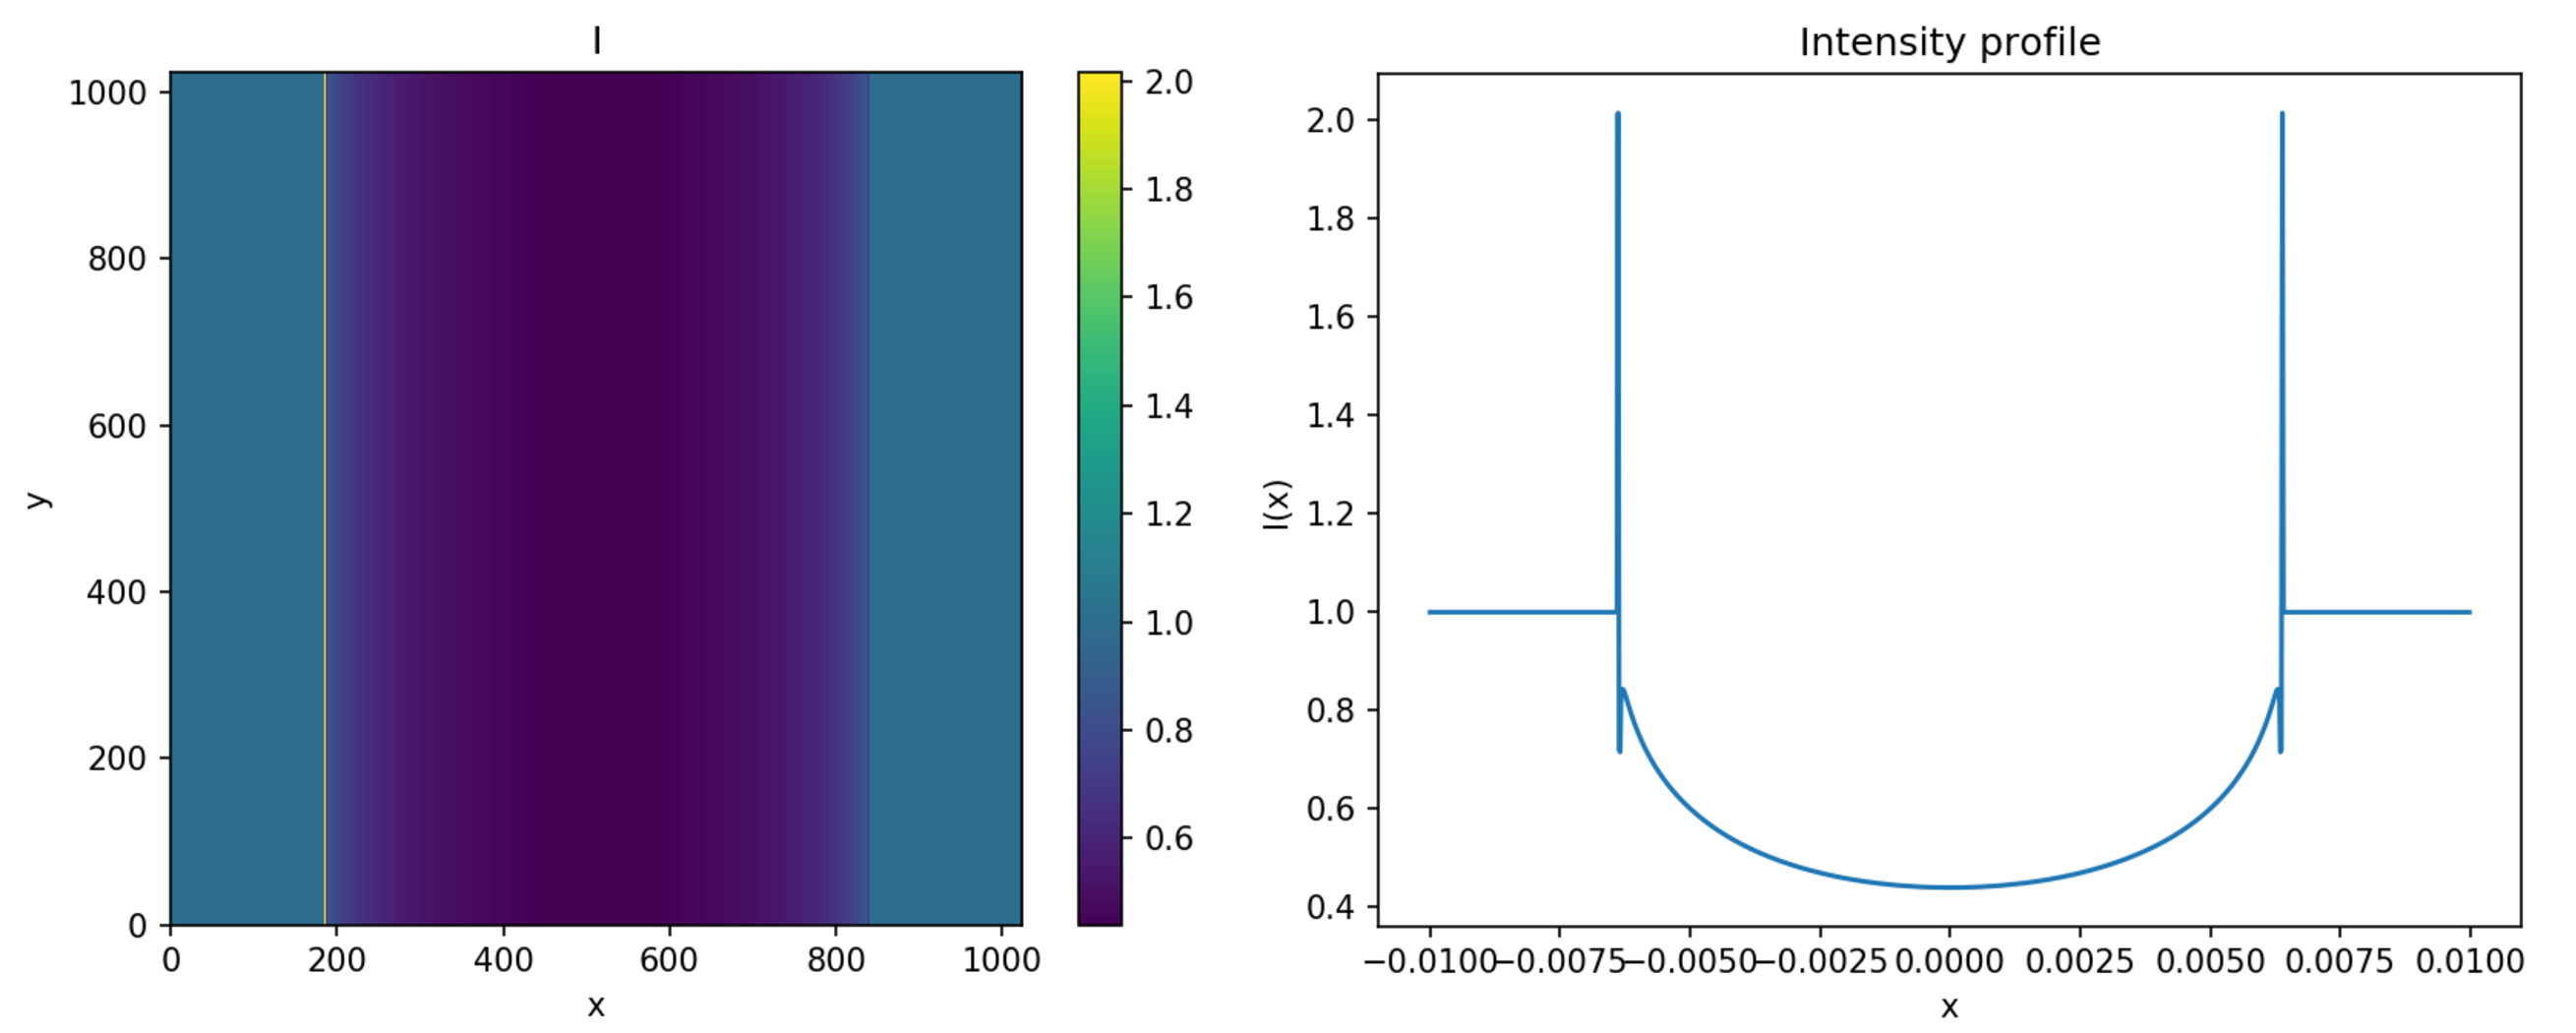
\includegraphics[width=\linewidth]{FD_intensity_profile.pdf}
\captionof{figure}{These phase contrast image and phase contrast cross section were obtained using my non-Fourier method. As it can be seen here the phase contrast peaks are much higher than the profile found using the Fourier method. The parameters used to obtain this image were an X-ray energy equal to $22.1629$keV (corresponding to a Ag k-alpha 1 source), the cylinder's material was water which has a refractive index decrement $\delta_1 = 468.141$ nm while the attenuation coefficient at this energy is $\mu_1 = 64.38436\mathrm{m^{-1}}$, the sigmoid function blurred 0.14 pixels over the edge of the imaged cylinder. The apparent asymmetry of the two-dimensional phase contrast image is due to aliasing.}
\end{Figure}

% Therefore my first simulation will be that of a single monomorphic cylinder, 

2 cylinders
MK’s earlier comments:
We want to see:
a) whether density changes alone will give phase contrast and (as I think they will), how small the fringes will be;
b) how the fringes change when we start changing the spectrum. 
Of course for part b) we'll really need to use the angular spectrum or Fresnel codes, so you'll need those libraries working.
Adapting my code to match the refractive indices and attenuation coefficients of two concentric cylinders
 blah blah


% and later on I will work on 2 cylinders, one embedded on another, both these cylinders will have different densities, since I want to understand how much density difference is needed before I see phase contrast in my simulation.
% To solve the transport-of-intensity equation (TIE) and go beyond the projection approximation I have designed a differential equation solver using the fourth order Runge-Kutta algorithm. Since there is an intrinsic link between the phase and the TIE, I decided to solve re-write equation (\ref{eq:15}) in differential form and solve it simultaneously to the TIE in my code.
% So far I have been able to recover the phase gained by the incident X-ray wave-fronts as they cross the cylindrical material I simulated.
% \subsubsection{Results}
% \begin{Figure}
% \centering
% 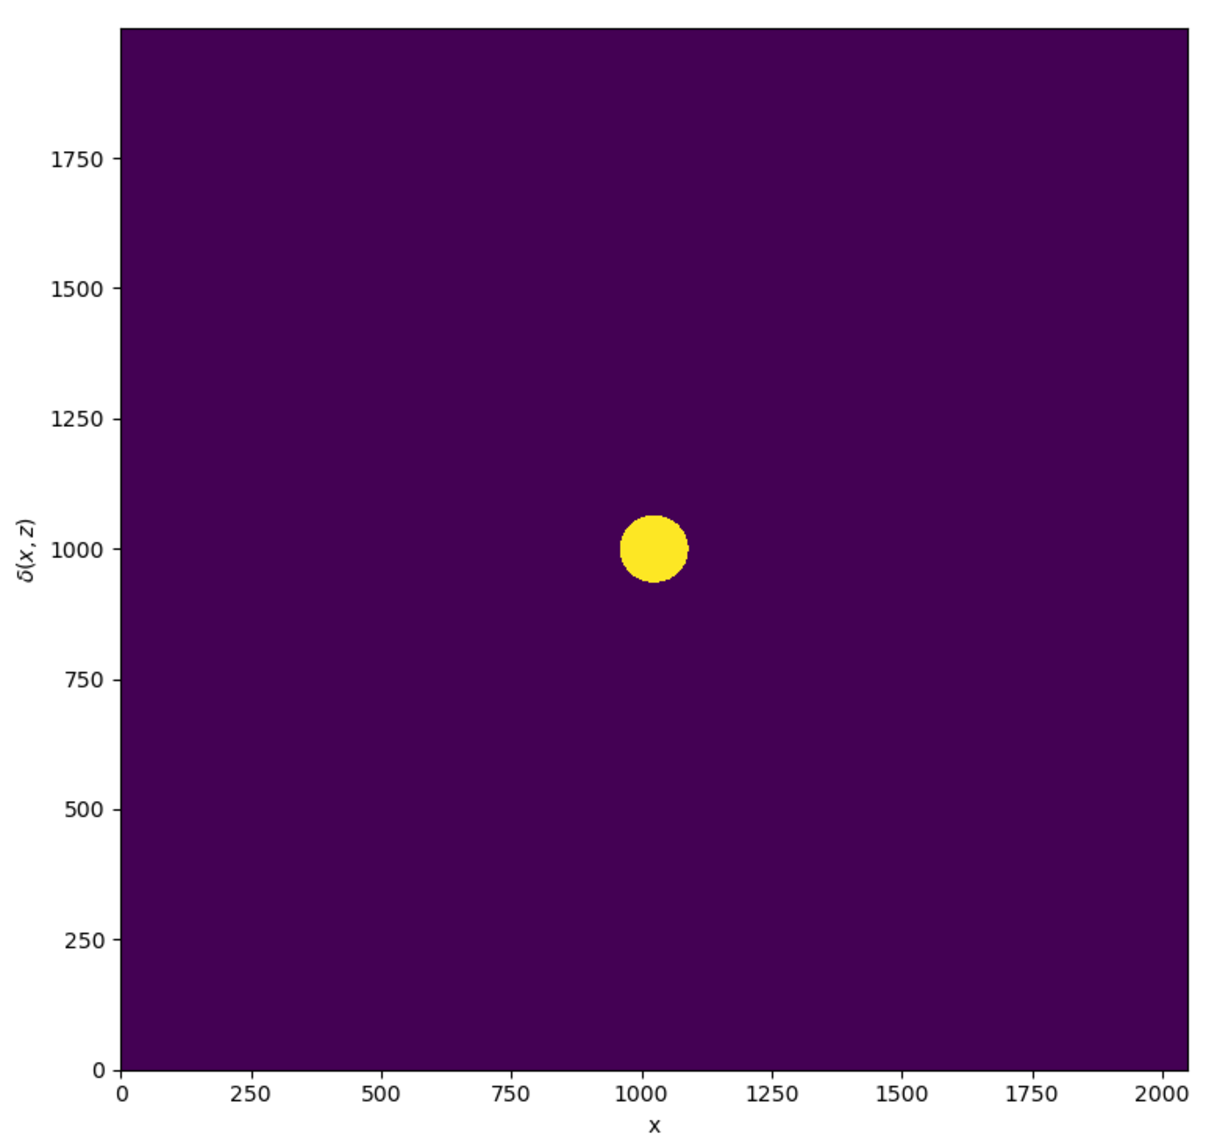
\includegraphics[width=0.6\linewidth]{cross_section.pdf}
% \captionof{figure}{I made this 2D plot to verify that the cross-sectional are a of my simulated cylinder did indeed reflect the correct geometry. Here one can see a purple background representing the complex refractive index value of the vacuum $\delta = 0$ and that of the cylinder in yellow $\delta_0 = 462.8 \times 10^{-9}$ (as was reported in \cite{Beltran} for the PERSPEX sample).}
% \end{Figure}
% \begin{Figure}
% \centering
% 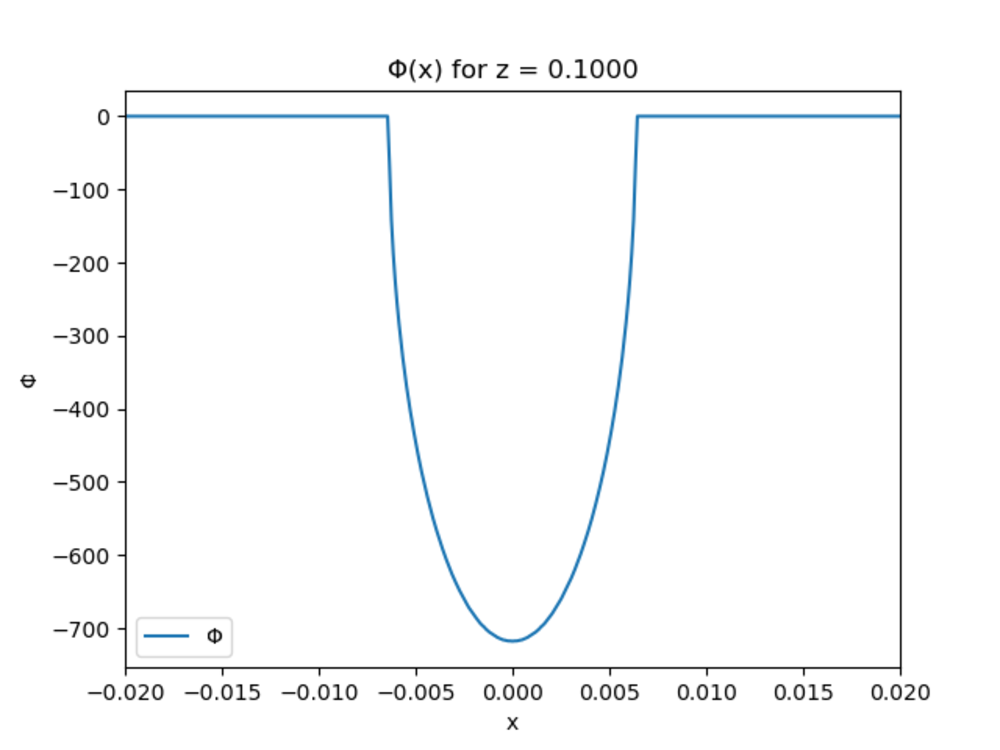
\includegraphics[width=0.6\linewidth]{20000.pdf}
% \captionof{figure}{The position-dependent phase shift I discovered by using fourth order Runge-Kutta.}
% \end{Figure}

\section{Future Plans}
% I aim to finish my simulation by creating a graphic user interface (GUI) that allows the user to modify interactively the density parameters of the imaged concentric cylinders in the simulation. The goal is to make a easily operated visual representation of the changes in phase and intensity of the X-rays as they interact with the object in-situ.

% In the foreseeable future my supervisor and I plan to diversify my project by making me do some simulations about a topic known as speckle analysis. A speckle pattern is commonly produced by interference of coherent light wave-fronts as these transmit through or reflect from a random phase assigning object (scattering medium), the process is known to encode information about the scattering medium that created the speckle\cite{Specks}. The main goal of making me do the speckle simulations is for me to understand the possible sources and causes of speckles in X-ray imaging, and to be able to decode speckle patterns.

% I also plan to aid my supervisor with testing a newly obtained silver target source of X-rays for his lab apparatus. I aim to do data analysis to compare the results from the new silver target to the classic tungsten target used in the apparatus currently.

\section{Conclusion}
% The present aim of my project is to create simulation to investigate how the phase of incident X-rays changes as the density of a sample material in an arbitrary imaging system changes. My investigation will be extended by simulating two distinct materials under the same wave-field and see if and how distinctly phase contrast occurs. The eventual goal of this simulation is to verify if successful phase retrieval can be done of the imaged objects given their variable densities. In this report I present a brief outline of the theoretical perspective of coherent X-ray imaging, a description of my current progress and future aims.

\bibliography{mybib}
\bibliographystyle{unsrt}
\end{document}
